\chapter{Introduction}

Submarine operators detect the presence of vessels in the surrounding waters primarily through the use of SOund Navigation and Ranging (sonar), a technology that leverages the propagation of sound waves through water to analyse the presence, location, and characteristics of underwater objects \cite{niu_advances_2023}. Sonar works analogously to how audio recording works in air: sound is carried through the water medium as longitudinal waves with a certain frequency and energy, and this pressure is picked up by a recording device called a hydrophone. These hydrophones convert the mechanical energy of the wave into an electrical signal, which can then be analysed using a variety of methods in the field of \acrfull{dsp} \cite{waite_sonar_2002, domingos_survey_2022}.

Classifying an object based on its sonar signature, a task known as underwater acoustic classification or \acrfull{uatr}, is a difficult job. This process is traditionally split into two stages: feature extraction and classification. Feature extraction focuses on identifying and isolating key attributes from raw sonar signals, while classification involves applying various models to categorise the input signals based on these extracted features (see Figure \ref{fig:luo-flowchart}). Currently, both these tasks are being undertaken by teams of highly-trained sonar technicians around the world \cite{aslam_underwater_2024}. These teams use large databases of patterns and signals collected from known objects over the years to compare and classify a new incoming signal \cite{niu_advances_2023}. It is a slow and cumbersome task which at present relies on traditional rule-based learning techniques \cite{neupane_review_2020}.  However, with recent advancements in artificial intelligence, researchers aim to automate \acrshort{uatr}, making it faster and potentially more accurate \cite{aslam_underwater_2024, neupane_review_2020}. Improving this automation of \acrshort{uatr} is the primary focus of this thesis.

\begin{figure}[htbp]
\centering 
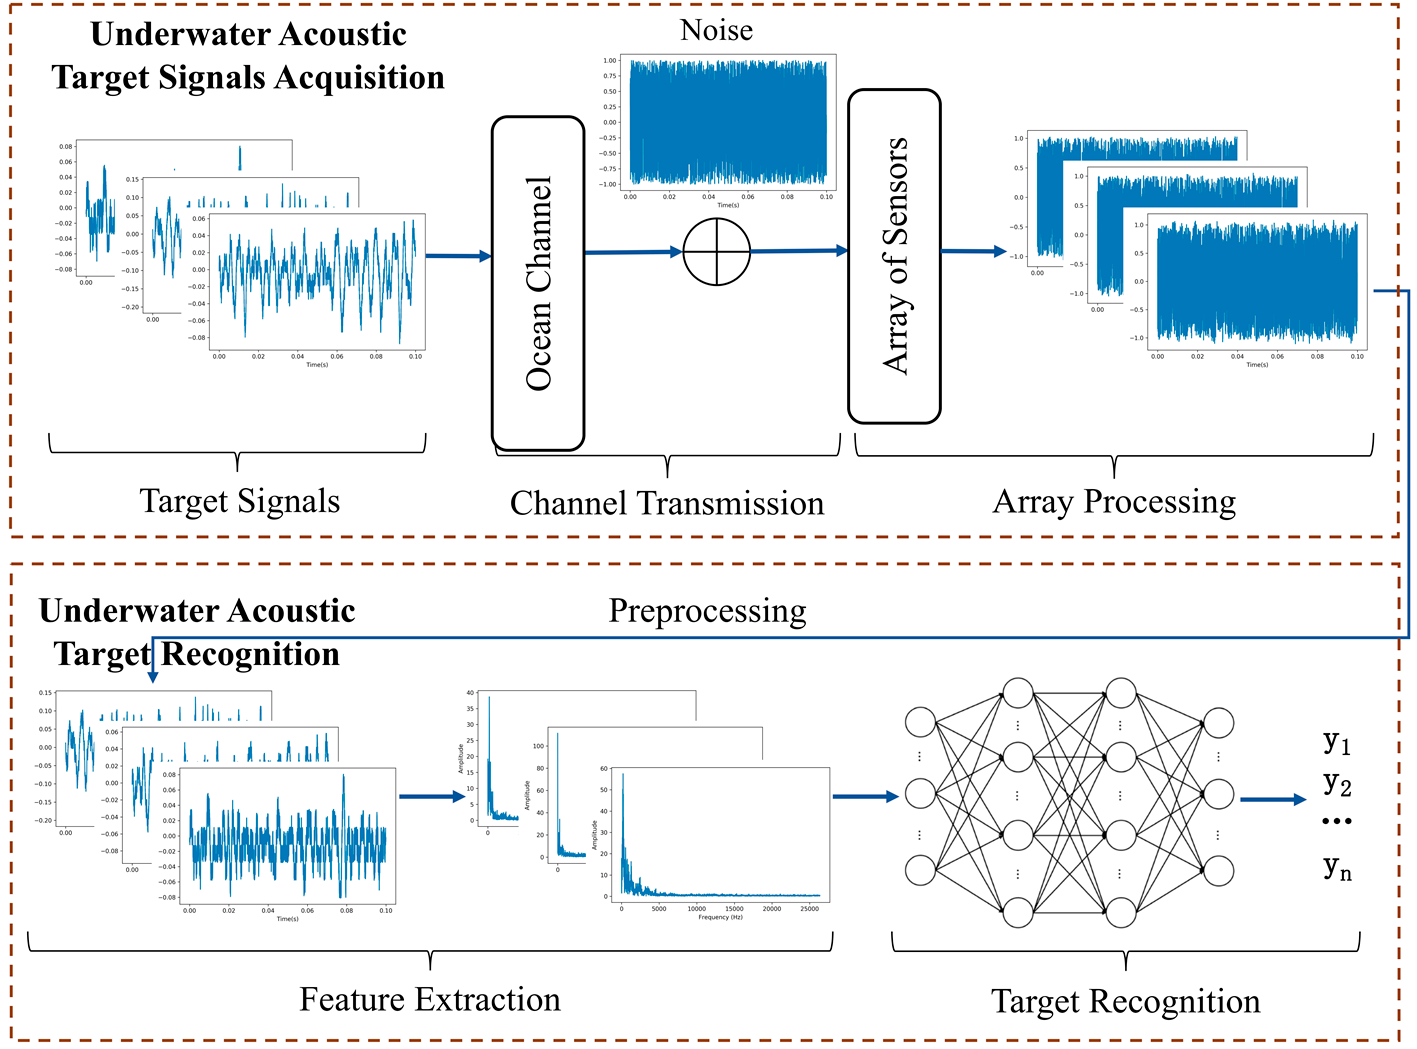
\includegraphics[width=0.9\textwidth]{img/ch1/flowchart.png} 
\caption{Flow chart of underwater acoustic signal acquisition and target recognition, obtained from \cite[Fig.~1]{luo_survey_2023}} 
\label{fig:luo-flowchart} 
\end{figure}

\section{Problem statement}

The underwater acoustic environment poses significant challenges due to its unpredictable and noisy nature. Factors such as signal reflection, refraction, and attenuation, along with diverse noise sources like marine life, vessel traffic, and environmental disturbances, create highly variable recordings. These conditions obscure meaningful features in sonar signals, making accurate classification for underwater acoustic target recognition (\acrshort{uatr}) a complex task. Without effective preprocessing, machine learning models tasked with classification are often overwhelmed by irrelevant noise, resulting in reduced accuracy and reliability.

Preprocessing techniques, including normalisation, detrending, and denoising, are essential for improving the quality of sonar signals. These methods reduce noise, suppress irrelevant trends, and emphasise key signal features, enhancing the effectiveness of downstream classification tasks. Despite their importance, limited research has systematically explored the role of traditional preprocessing techniques in the context of modern deep learning-based \acrshort{uatr}. The unique challenges of the underwater domain, such as limited labelled datasets and the inherent variability of sonar signals, demand a tailored investigation into how preprocessing can enhance feature representations for classification.

This thesis aims to address this gap by exclusively focusing on preprocessing techniques to enhance input features for \acrshort{uatr}. Specifically, it systematically evaluates the impact of normalisation, detrending, and denoising on the performance of a benchmark CNN-LSTM classifier.

\section{Proposed solution}

In this work, normalisation techniques such as channel-based and global normalisation are assessed for their ability to standardise spectrogram inputs and improve model performance. The $\ell_1$ detrending algorithm is explored for its potential to remove long-term trends, emphasising short-term variations that may contain critical target characteristics. Finally, denoising experiments investigate noise reduction frameworks, including the Noise2Noise methodology and masking-based techniques, to determine their efficacy in isolating relevant features in noisy underwater acoustic environments. By applying these preprocessing methods in a controlled experimental setup, this thesis quantifies their contributions to \acrshort{uatr} accuracy and robustness, offering insights into their effectiveness and limitations for this challenging domain.

All source code for this thesis can be found at \url{https://github.com/antrikshdhand/thesis/tree/main}.

\section{Outline}

The structure of this thesis is as follows:

\paragraph{Chapter 2: Background and Literature Review} This chapter provides essential theoretical background for readers, covering key aspects of underwater acoustic signal propagation, such as noise sources and their impact on signal quality, which are relevant for the denoising work explored later. The chapter also offers an introduction to artificial intelligence and concludes with a comprehensive literature review, summarising over 50 foundational and recent high-impact studies within the field.

\paragraph{Chapter 3: Establishing a Benchmark Performance} Here, the CNN-LSTM architecture is established as the benchmark classifier model for our experiments with a detailed description of its inputs, structure, configuration, and baseline performance metrics. This architecture serves as a point of reference for evaluating all subsequent preprocessing techniques.

\paragraph{Chapter 4: Normalisation}
This chapter explores the impact of normalisation techniques on \acrshort{uatr} performance. It evaluates channel-based and global normalisation strategies to determine their effect on standardising spectrogram inputs and improving the accuracy and stability of the CNN-LSTM model. Findings highlight the importance of aligning preprocessing techniques with the specific characteristics of the dataset.

\paragraph{Chapter 5: Detrending} 
The role of detrending in \acrshort{uatr} is investigated in this chapter, focusing on the $\ell_1$ detrending algorithm. By removing long-term trends from acoustic spectrograms, the experiment aims to suppress irrelevant noise and enhance transient features critical for classification. The impact of various detrending strengths is evaluated, with results revealing the limitations and potential disruptions caused by this technique.

\paragraph{Chapter 6: Denoising}
This chapter examines denoising methods for underwater acoustic spectrograms, with a focus on the Noise2Noise framework and masking-based techniques. It evaluates the effectiveness of these methods and highlights the challenges of adapting image-based denoising frameworks to the underwater domain.

\paragraph{Chapter 7: Conclusion}
The final chapter synthesises the findings of the thesis, summarising the contributions and limitations of the preprocessing techniques investigated.